\hypertarget{asynchrone-cryptography}{%
\section{Asynchrone Cryptography}\label{asynchrone-cryptography}}

\textbf{Repetition:} \\
P: set of possible plain texts  \\
C: set of possible cipher texts \\
K: finite set of possible keys 
E: finite set of encryption functions\\
$E_k : P \Rightarrow C, k \in K \\$
D: finite set of decryption functions\\
$D_k : C \Rightarrow P, k \in K$
For every e $\in$ K there is a d $\in$ K such that\\
$D_d (E_e(p) = p$ for every $p \in P$

\hypertarget{symmetrische-verschluxfcsselung}{%
\subsection{Symmetrische
Verschlüsselung}\label{symmetrische-verschluxfcsselung}}

\begin{itemize}
\tightlist
\item
  Symmetric Cryptosystem

  \begin{itemize}
  \tightlist
  \item
    Uses basically the same key to encrypt and to decrypt. (Key d for decryption can be computed easily from the key e for encryption)
  \end{itemize}
\item
  Problems

  \begin{itemize}
  \tightlist
  \item
    Key must be kept secret!
  \item
    Each pair of users needs another secret key $\Rightarrow$ number of keys grows
    with $n^2$
  \end{itemize}
\end{itemize}

\hypertarget{asymmetrische-verschluxfcsselung}{%
\subsection{Asymmetrische
Verschlüsselung}\label{asymmetrische-verschluxfcsselung}}

\hypertarget{idea}{%
\subsubsection{Public Key Crypto System}\label{idea}}

\begin{figure}[H]
\centering
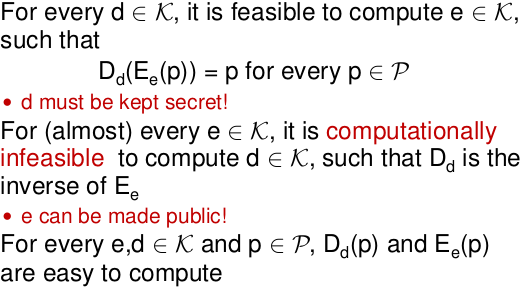
\includegraphics[width=0.5\textwidth]{figures/publicKeyIdea.png}
\caption{Idea of Public Key Crypto System}
\end{figure}

\begin{itemize}
\tightlist
\item
  Aus dem Entschlüsselungsschlüssel, kann ich einfach den Schlüssel zum
  Verschlüsseln berechnen
\item
  Aber aus dem Verschlüsselungsschlüssel kann ich nicht (inner
  nützlicher Frist) den Entschlüsselungsschlüssel berechnen.
\item
  Da niemand aus dem Schlüssel E den Schlüssel D berechnen kann, kann
  ich den Schlüssel E publizieren.
\end{itemize}

\subsubsection{One-Way-Function}
\textbf{Wir suchen also etwas wie eine Einweg-Funktion:} 
\begin{itemize}
    \item One-way function
    \begin{itemize}
        \item Easy to compute on every input (polynomial time)
        \item Hard to invert, given the image of a random input (Any polynomial time algorithm that tries to find an input that produces a given image will almost always fail)
        \item \textbf{Existence of one-way functions is still a conjecture!}
    \end{itemize}
    \item Trapdoor function
    \begin{itemize}
        \item One-way function that can be inverted if a secret is known
    \end{itemize}
\end{itemize}

\hypertarget{candidates-of-one-way-functions}{%
\subsubsection{Candidates of one-way
functions}\label{candidates-of-one-way-functions}}

\begin{itemize}
\tightlist
\item
  Multiplication and factoring

  \begin{itemize}
  \tightlist
  \item
    Easy: given two primes p and q compute $n = p*q$
  \item
    Difficulty: given $n = p*q$, find the two primes $p$ and $q$
  \end{itemize}
\item
  Discrete Logarithm Function

  \begin{itemize}
  \tightlist
  \item
    Easy: given $g, x$ and $p$, compute $g^x \mod p$
  \item
    Difficult: given $g^x \mod p$, $g$ and $p$, find $x$
  \end{itemize}
\item
  Elliptic Curves (see later)

  \begin{itemize}
  \tightlist
  \item
    Easy: given the point $P$ and $n$, compute $n*P$
  \item
    Difficult: given $n*P$ and $P$, compute $n$
  \end{itemize}
\end{itemize}

\hypertarget{diffie-hellman-key-exchange}{%
\subsection{Diffie-Hellman Key
Exchange}\label{diffie-hellman-key-exchange}}

\begin{figure}[H]
\centering
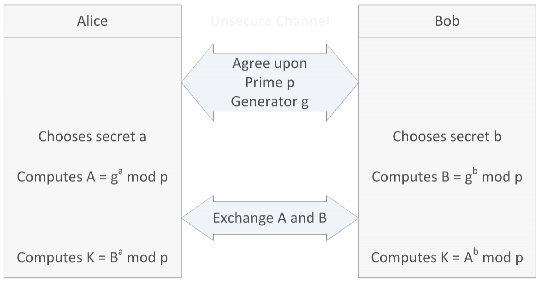
\includegraphics[width=0.65\textwidth]{figures/dhke.png}
\caption{Diffie-Hellman Key-Exchange}
\end{figure}

\begin{itemize}
    \item If you know how to compute the discrete logarithm, DHKE is broken (no algorithm is known)
    \item Man-in-the-middle attack
    \item You have to be sure that the messages are authentic. Otherwise Eve could exchange a secret key with both Alice and Bob
\end{itemize} 

\subsection{ElGamal Encryption}
\subsubsection{Key generation}
\begin{enumerate}
    \item Alice chooses prime p and generator g
    \item Alice chooses an exponent $1 \leqslant a \leqslant p - 2$ randomly and computes $A = g^a \mod p$
    \item Alices publishes (p, g, A) as her public key
\end{enumerate}

\subsubsection{Encryption}
\begin{enumerate}
    \item Bob get Alices public key (p, g, A)
    \item Bob chooses a random number $1 \leqslant b \leqslant p - 2$ and computes $B = g^b \mod p$
    \item For the message m, Bob computes the cipher text $c = A^b * m \mod p$
    \item Bobs secret message consists of B and c
\end{enumerate}

\subsubsection{Decryption}
\begin{enumerate}
    \item Alice computes $B^{(p - 1 - a)} * c \equiv m \mod p$
\end{enumerate}

\subsection{RSA}
\subsubsection{Key Generation}

\begin{enumerate}
    \item Choose randomly two (large) primes $p, q$ and compute $n = p*q$
    \item Choose an integer $1 < e < \varphi(n)$ such that $gcd(e, \varphi(n)) = 1$
    \begin{itemize}
        \item Note: $\varphi(n) = (p - 1)*(q - 1)$ can easily be computed if you know $p$ and $q$ 
    \end{itemize}
    \item Find $d$ such that $e*d \equiv 1 (\mod \varphi(n))$
    \begin{itemize}
        \item Since $gcd(e, \varphi(n)) = 1$ such an integer exists
        \item Use Euclid's extended algorithm
    \end{itemize}
    \item Publish ($e, n$), keep $d$ secret
\end{enumerate}

\emph{e steht für encryption und ist der öffentliche Schlüssel.}

\hypertarget{encryption-decryption}{%
\subsubsection{Encryption \& Decryption}\label{encryption-decryption}}

\begin{itemize}
\tightlist
\item
  Encryption

  \begin{itemize}
  \tightlist
  \item
    Map the plain message $M$ to one (or several) integers $0 \leqslant m < n$
  \item Compute cipher text $c = m^e \mod n$
    \begin{itemize}
    \tightlist
    \item
      Note since $e$ is public, everybody can do that
    \end{itemize}
  \end{itemize}
\item
  Decryption
  \begin{itemize}
  \tightlist
  \item
    Compute $m' = c^d \mod n$
    \begin{itemize}
    \tightlist
    \item
      We claim that $m' = m$
    \item
      Note since $d$ is private, only the authorized recipient can do that
    \end{itemize}
  \end{itemize}
\end{itemize}

\hypertarget{square-and-multiply}{%
\subsection{Square and Multiply}\label{square-and-multiply}}

Zum Ausrechnen von natürlichen Potenzen $x^k, k \in N$.
\begin{itemize}
    \item k in eine binäre Zahl umwandeln
    \item Jede 0 durch Q ersetzen, jede 1 durch QM ersetzen
    \item Das QM ganz links streichen
    \item Von links nach rechts arbeiten
    \begin{itemize}
        \item Für jedes Q das aktuelle Resultat quadrieren
        \item Für jedes M das aktuelle Resultat mit x multiplizieren
        \item Nach jedem Schritt kann der Modulo angewendet werden
    \end{itemize}
\end{itemize}

\begin{tcolorbox}[colback=red!5!white,colframe=red!75!black]
    \textbf{Beispiel} \\
    $3^{21} \mod 11 =$ ? \\
    $21_d = 10101_b \Rightarrow $ \sout{$QM$}$QQMQQM$ \\
    $Q: 3^2 = 9 \mod 11 \equiv 9$ \\
    $Q: 9^2 = 81 \mod 11 \equiv 4$ \\
    $M: 4*3 = 12 \mod 11 \equiv 1$ \\
    $Q: 1^2 = 1 \mod 11 \equiv 1$ \\
    $Q: 1^2 = 1 \mod 11 \equiv 1$ \\
    $M: 1*3 = 3 \mod 11 \equiv 3$
\end{tcolorbox}

\hypertarget{primality-testing}{%
\subsection{Primality Testing}\label{primality-testing}}

\begin{itemize}
    \item Let n be an integer
    \item Suppose there exist integers $x$ an with $x^2 \equiv y^2 \mod n$, but $x \neq +-y \mod n$
    \item Then $n$ is composite and $gcd(x - y, n)$ gives a nontrivial factor of $n$
\end{itemize}
Mit anderen Worten

\begin{itemize}
\tightlist
\item
  Ich gebe Ihnen eine Zahl n
\item
  Wenn es Ihnen gelingt, ein X und ein Y zu finden, mit folgenden
  Eigenschaften
  \begin{itemize}
  \tightlist
  \item
    $X \neq Y$
  \item
    $X \neq-Y$
  \item
    $x^2 \equiv y^2 \mod n$
  \end{itemize}
\item
  Dann ist $n$ keine Primzahl. $\Rightarrow$ Es gibt Teiler in $gcd(x-y,n)$
\end{itemize}

\hypertarget{miller-rabin---basic-idea}{%
\subsubsection{Miller-Rabin - Test}\label{miller-rabin---basic-idea}}

\begin{figure}[H]
\centering
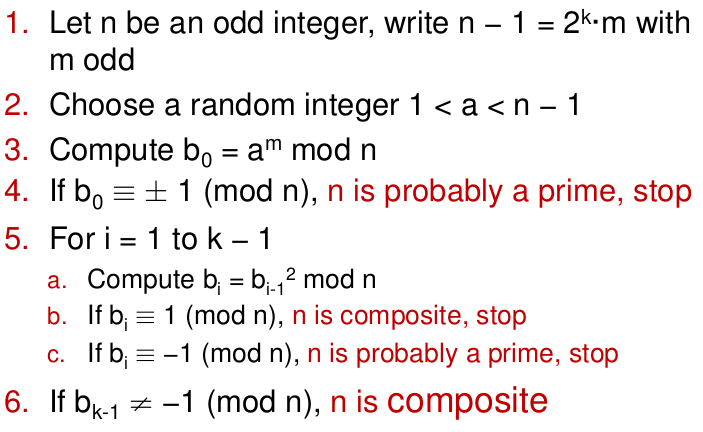
\includegraphics[width=0.7\textwidth]{figures/Miller-Rabin-Algorithmus.png}
\caption{Miller-Rabin Test}
\end{figure}

\textbf{Algorithmus:}

\begin{itemize}
\tightlist
\item
  Wenn n eine Primzahl ist, dann besteht sie den Test für jedes a
\item
  Wenn n keine Primzahl ist, dann besteht sie den Test mit einer
  Wahrscheinlichkeit von $1/4$
\item
  Wenn man den Test $M$ mal wiederholt, ist die Wahrscheinlichkeit, dass
  $n$, wenn sie keine Primzahl ist, den Test besteht bei $(1/4)^M$
\end{itemize}

\clearpage
\hypertarget{attacken-auf-den-rsa}{%
\subsection{Attacken auf den RSA}\label{attacken-auf-den-rsa}}

\begin{itemize}
\tightlist
\item
  Let $n = p*q$ have $m$ digits. If we know the first $m/4$ or the last $m/4$
  digits of $p$, we can efficiently factor $n$ Choose $p$ (and $q$) such that a
  large amount of $p$ is not predictable
  \begin{itemize}
  \tightlist
  \item
    \textbf{Bedeutet $p$ und $q$ müssen zufällig und gross gewählt werden}
  \end{itemize}
\item
  Suppose $(e,n)$ is an RSA public key and $n$ has $m$ digits. Let $d$ be the
  private key. If we have at least the last $m/4$ digits of $d$, we can find
  $d$ in time that is linear in $e*log_2(e)$

  \begin{itemize}
  \tightlist
  \item
    If $e$ is large (around $n$) this is not better than a case-by-case search
  \end{itemize}
\end{itemize}

\hypertarget{small-public-exponent}{%
\subsubsection{Small Public Exponent}\label{small-public-exponent}}

\begin{itemize}
\tightlist
\item
  Suppose the same message $m$ is encrypted with the same (small) public exponent $e$ but different modulo $n_1, n_2$, \ldots{}, $n_e$
  \begin{itemize}
  \tightlist
  \item
    $c_1 = m^e \mod n_1, c_2 = m^e \mod n_2, \ldots{}, c^e = m^e \mod n^e$
  \end{itemize}
\item
  Use Chinese Remainder Theorem to compute $c$ with $c \equiv c_i \mod n_i$ and $0 \leqslant c < n_1 * n_2 * \ldots{} *n_e$
\item
  We claim that $c = m^e$ (without modular reduction!)
\item
  We may find $m$ by computing $m = c^{1/e}$

  \begin{itemize}
  \tightlist
  \item
    Note: this is possible, because we do not use modular arithmetic
  \end{itemize}
\end{itemize}

Also wenn für mehrere Nachrichten derselbe öffentliche Schlüssel verwendet wurde und dieselbe Nachricht m verschlüsselt wird, können wir den \textbf{chinesischen Restwertsatz} verwenden, um ein passender geheimer Schlüssel zu errechnen.

\begin{tcolorbox}[colback=red!5!white,colframe=red!75!black]
\textbf{Beispiel:} \\
Suppose we know $c_1 = 60, c_2 = 203, c_3 = 711$ and $n_1 = 143, n_2 = 391, n_3 = 899$ and $e = 3$ \\
With the CRT find c with $c \equiv 60 \mod 143, c \equiv 203 \mod 391, c\equiv 711 \mod 899 \Rightarrow c = 2460375$ \\
We compute the message $m = c^{1/e} = 2460375^{1/3} = 135$
\end{tcolorbox}

\clearpage